\documentclass[../main.tex]{subfiles}
\graphicspath{{\subfix{../img/}}}

\begin{document}

\thispagestyle{empty}
\etocignoretoctocdepth % of course, if we want to see something in local TOC...
\etocsettocstyle{\subsection*{\contentsname}}{}
\localtableofcontents
\newpage
\setcounter{page}{1}

%%%%%%%%%%%%%%%%%%%%%%%%%%%%%%%%%%%%%%%%%%%%%%%%%%%%%%%%%%%%%%%%%%%%%%%%%%%%%%%%%
\color{red}

From a dynamical systems perspective, bursting can arise through a variety of
mechanisms, including stable limit cycles, chaotic attractors, canard-induced
mixed-mode oscillations, and other complex nonlinear dynamics.

\color{black}

%%%%%%%%%%%%%%%%%%%%%%%%%%%%%%%%%%%%%%%%%%%%%%%%%%%%%%%%%%%%%%%%%%%%%%%%%%%%%%%%%
\section{Conductance Based Models For Bursting Neurons}

\subsection{Preface}

Generally, any model neuron that can spike can also burst under modeulation of
time-dependent external input $I(t)$ \cite{izhikevichDynamicalSystemsNeuroscience2006}
(\textbf{\textit{forced burster}}, Fig. \ref{fig:example_forced_intrinsic_bursters}a).
However, a neuron can also burst intrinsically under constant input due to the interplay
between ionic currents mediated by ion channels present in the membrane of the neuron
(\textbf{\textit{intrinsic burster}}, Fig. \ref{fig:example_forced_intrinsic_bursters}b).
Although it is known whether R5 neurons are intrinsic bursters or not
\cite{raccugliaNetworkSpecificSynchronizationElectrical2019}, as \gls{swa}
is thought to be generated at the level of R5 \cite{raccugliaNetworkSpecificSynchronizationElectrical2019},
in the current work it will be assumed, that R5 neurons exhibit bursting behavior
due to intrinsic properties, rather than via time-varied external input.

Resting and spiking states, as well as transition between them can exhibit different
features for different models. The examples of bursting neurons in Figures
\ref{fig:ionic_basis_for_slow_fast_bursting}
and \ref{fig:example_forced_intrinsic_bursters} illustrates the case when the resting
state is a stable equilibrium and spiking state is limit cycle attractor. However,
generally, the resting state can also be a limit cycle attractor (not shown here).
As the eleqtrophysiological recordings of R5 neurons do not show subthreshold oscillations
at resting state, this case will be omitted in this chapter. The case when the resting state
is a stable equilibrium is referred to as \textbf{\textit{'point-cycle burster'}}
\cite{izhikevichNEURALEXCITABILITYSPIKING2000}, and will be the main focus in the following.
For simplicity, unless stated otherwise, this type of bursting will be referred to as 'bursting'.


%%%%%%%%%%%%%%%%%%%%%%%%%%%%%%%%%%%%%%%%%%%%%%%%%%%%%%%%%%%%%%%%%%%%%%%%%%%%%%%%%
\subsection{Ohmic vs \texorpdfstring{\gls{ghk}}{GHK} Current}

The current through an ion channel can be modelled useing either Ohm's law, or
\gls{ghk} current equation. Ohmic current assumes linear relationship between
voltage and conductance \textcolor{red}{Citation}:
\begin{equation}\label{eq:ohmic_current}
    I_{c}(V,t) = g_c(V,t)(V - V_c)
\end{equation}
where $V$ is membrane potential, $g_c(V,t)=\bar{g_c}m^p(V,t)h^q(V,t)$ is conductance calculated
as a product of maximal conductance and probabilities of activation ($m$) and
inactivation ($h$) gates being open, $V_c$ is reversal potential. Here, the
concentration between the extracellular and intracellular ion concentrations
is hidden inside $V_c$
(see Equation \ref{eq:nernst_equation} in Section \ref{subsubsec:ion_channel_properties_and_function}
for the case when an ion channel is permeable to one ion).
\gls{ghk} equation on the other hand models nonlinear relationship between the variables in
explicit way \textcolor{red}{Citation}:
\begin{equation}\label{eq:ghk_current}
    I_c(V,t) = g_c(V,t) P z^2 \frac{VF^2}{RT}\frac{[\text{ion}]_{\text{inside}} - [\text{ion}]_{\text{outside}} \exp{[-zFV/(RT)]} }{1 - \exp{[-zFV/(RT)]}}
\end{equation}
where, $P$ is permeability, $R$ is the universal gas constant ($8315$ mJ/(K$^\circ$$\cdot$Mol)), $T$ is temperature measured
in Kelvin, $F$ is Faraday's constant ($96480$ coulombs/Mol), $z$ is the valence of the ion,
whereas $[\text{Ion}]_{\text{in}}$ and $[\text{Ion}]_{\text{out}}$ are ion concentrations inside and outside membrane.

Equation \ref{eq:nernst_equation} can be obtained from \ref{eq:ghk_current} if one considers
equilibrium condition, whre the ionic current $I_c=0$. Nernst equation assumes that ion concentrations
are fixed. However, Equation \ref{eq:ohmic_current} can be still used when ion concentration dynamics
are incorporated in the model by recalculating reversal potential at each stimulation step.

For some ion channels Equation \ref{eq:ohmic_current} is sufficient to reproduce experimentally obtained
voltage-current relationships. However, for other channels Ohmic current does not provide good
estimates and \gls{ghk} current equation should be used to obtain better fit between
experimental data and simulations \textcolor{red}{Citation} (see also \textcolor{red}{Section ???} for
\textit{Drosophila} T-type $Ca^{2+}$ ion channels).

%%%%%%%%%%%%%%%%%%%%%%%%%%%%%%%%%%%%%%%%%%%%%%%%%%%%%%%%%%%%%%%%%%%%%%%%%%%%%%%%%
\subsection{Bifurcations in fast-slow subsystems}

Bifurcation analysis is a powerfull tool to investigate the behavior of
a dynamical system. Specifically, how given system switches between
different states when one or multiple parameters (referred to as \textbf{bifurcation parameters})
are varied. As it will be evident throughout this section, the choice of the
bifurcation parameter is crucial and depends on
what aspects of the system one aims to investigate.

Within the framework of the fast-slow subsystems with single slow variable
one can consider the slow variable as a bifurcation parameter and investigate
how changing the value of that variable affects the state of the fast subsystem:
for what values is the fast subsystem at rest or spiking state and how does transition
between these states occur. Thus, when the mechanism of bursting is investigated,
one can divide the question into two parts: 1) What initiates a burst? 2) What terminates a burst?
Before getting deeper into possible mechanisms and suggesting what dynamical properties
R5 neurons may have, let us consider one example.

%%%%%%%%%%%%%%%%%%%%%%%%%%%%%%%%%%%%%%%%%%%%%%%%%%%%%%%%%%%%%%%%%%%%%%%%%%%%%%%%%
\subsubsection{Equivalent voltage and example of fast-slow decomposition}

\begin{figure}[!t]
    \centering
    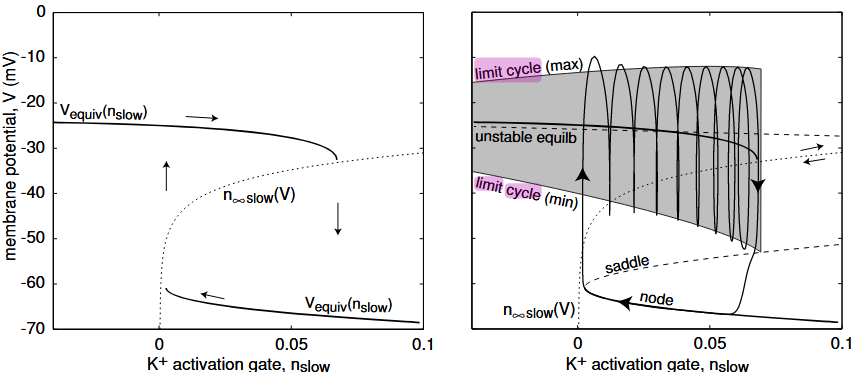
\includegraphics[width=0.85\linewidth]{../img/2_mathematical_overview/fast_slow_system_example.png}
    \caption[Example of fast-slow decomposition]{
        \textbf{Exampl of fast-slow decomposition}.
        Adapted from \cite{izhikevichDynamicalSystemsNeuroscience2006}.
        \textcolor{red}{Text}
    }
    \label{fig:example_fast_slow_decomposition}
\end{figure}

%%%%%%%%%%%%%%%%%%%%%%%%%%%%%%%%%%%%%%%%%%%%%%%%%%%%%%%%%%%%%%%%%%%%%%%%%%%%%%%%%
\subsubsection{Bifurcations of equilibria and cycles}

Burst initiation is transition
from resting (when the neuron does not fire action potentials) to spiking state,
referred to as \textbf{bifurcation of equilibria}.

Transition between spiking to
resting state is referred to as \textbf{bifurcation of cycles}
\cite{izhikevichNEURALEXCITABILITYSPIKING2000,izhikevichDynamicalSystemsNeuroscience2006}.

\begin{table}[h!]
    \centering
    \begin{tabular}{|c||c|c|c|c|}
        \hline
        Bifurcation of Equilibria & Behavior & Frequency & Amplitude & Operation \\ 
        \hline
        \hline
        Fold & bi-stable & nonzero & fixed & integrator \\
        \gls{snic} & excitable & zero ($\sqrt{\lambda}$) & fixed & integrator \\
        Supercritical Hopf & excitable & nonzero & zero ($\sqrt{\lambda}$) & resonator \\
        Subcritical Hopf & bi-stable & nonzero & arbitrary & resonator \\
        \hline
    \end{tabular}
    \caption[Bifurcations of Equilibria]{Bifurcations of Equilibria
    (adapted from \cite{izhikevichNEURALEXCITABILITYSPIKING2000} with modifications)}
    \label{tab:bifurcations_equilibria}
\end{table}

\begin{table}[h!]
    \centering
    \begin{tabular}{|c||c|c|c|}
        \hline
        Bifurcation of Cycles & Behavior & Frequency & Amplitude \\
        \hline
        \hline
        \gls{snic} & excitable & zero ($\sqrt{\lambda}$) & fixed \\
        Supercritical Hopf & excitable & nonzero & zero ($\sqrt{\lambda}$) \\
        Fold Limit Cycle$^{*}$ & bi-stable & nonzero & arbitrary \\
        Saddle Homoclinic Orbit & bi-stable & zero ($1/|\ln{\lambda}|$) & fixed \\
        Saddle-Focus Homoclinic Orbit & bi-stable & zero ($1/|\ln{\lambda}|$) & fixed \\
        Focus-Focus Homoclinic Orbit & bi-stable & zero ($1/|\ln{\lambda}|$) & fixed \\
        Subcritical Flip$^{**}$ & bi-stable & nonzero & arbitrary \\
        Subcritical Neimark-Sacker & bi-stable & nonzero & arbitrary \\
        Blue-sky & excitable & zero ($\sqrt{\lambda}$) & fixed \\
        \hline
    \end{tabular}
    \caption[Bifurcations of Cycles]{Bifurcations of Cycles
    (Adapted from \cite{izhikevichNEURALEXCITABILITYSPIKING2000} with modifications).
    $^{*}$Also called Saddle Node of Limit Cycles;
    $^{**}$Also called period-doubling bifurcation;}
    \label{tab:bifurcations_cycles}
\end{table}


%%%%%%%%%%%%%%%%%%%%%%%%%%%%%%%%%%%%%%%%%%%%%%%%%%%%%%%%%%%%%%%%%%%%%%%%%%%%%%%%%
\subsection{Preliminary Remarks}

\color{red}

\cite{golombContributionPersistentNa2006} - Example of bifurcation analysis 4+1 system

Gating mechanism - probability of ion channel to be in the open state

Bifurcation analysis helpful for: explaining why neuron stays for short period in bursting?
Why it is robust to perturbations or noise?

Example of transition from steady state to subthreshold oscillations with
increasing currents via Hopf bifurcation \cite{wangMultipleDynamicalModes1994}

Example of hopf \cite{golombContributionPersistentNa2006}

(Okay, so, if Ca concentration affects the bursting, maybe one should model Ca dependent channels with
Goldman-Hodgkin-Katz flux equation ??? It is even second argument for this equation, the first one being that
the fit is better!!!)
(Liu et al 2016)

Izhikevich - classification based on codimention 1 bifurcation

\color{black}

\begin{figure}[!b]
    \centering
    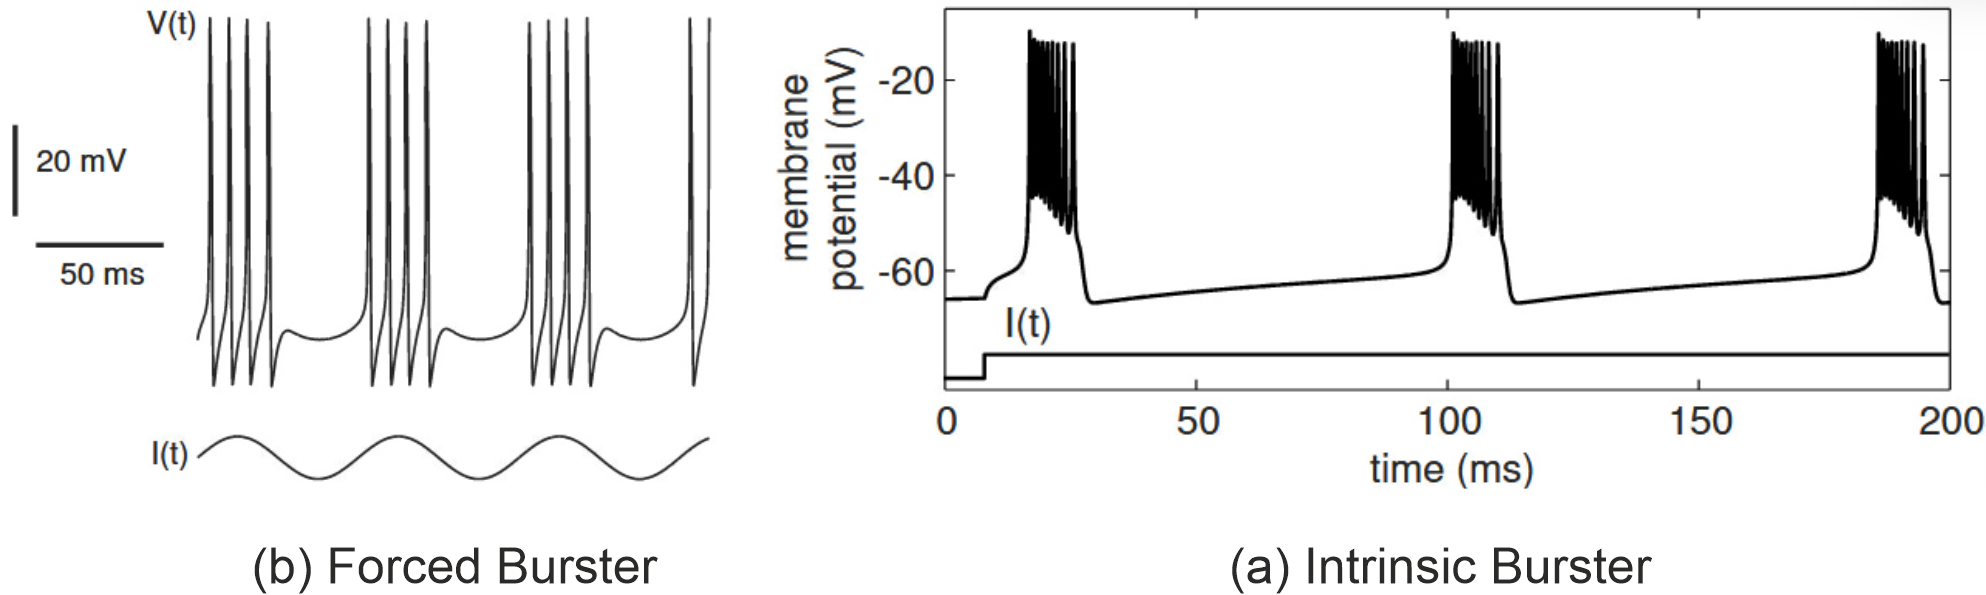
\includegraphics[width=0.85\linewidth]{../img/modelling_r5/examples/intrinsic_vs_forced_burster.png}
    \caption[Forced vs intrinsically bursting neurons]{
        Forced vs intrinsically bursting neurons. Examples of model neurons bursting due to time-varied external input (a) and intrinsic
        properties (b). Adapted from \cite{izhikevichDynamicalSystemsNeuroscience2006}, with modifications.
    }
    \label{fig:example_forced_intrinsic_bursters}
\end{figure}

\textcolor{red}{Write a few workds about the model in Lara's thesis -> it is not
biologically plausible model -> How can it be done with more biologically plausible model?
-> Generally, the distribuion of ion channels is different along neuron +
as it was stated in previos chapter, the soma thing. Here, for simplicity we start
from the single compartment neuonal model assuming uniform distribution of the
ion channels and ignoring the different compartments of the model.
Maybe in the discussion write that the morphology enhances robustness (there is a paper)
and maybe find some other pros for multicompartment models.
Citations: Laura \cite{krummSlowlyOscillatingBrain2021}
Richards manuscript \cite{raccugliaCoherentMultilevelNetwork2022}
}

The aim of the current work is to prupose a biologically pausible model for R5 neurons
to explain \textcolor{red}{what is written in the previous paragraph}.

Different models and approaches have been proposed to study bursting neurons.



One way to study the bursting neurons is to decompose the system into fast and
slow subsystems. Here, the fast subsystem corresponds to the spiking state, whereas the slow
subsystem acts as the mechanism for the transition between spiking and resting states.
Furthermore, based on slow-fast system, neurons can be classified according to
corresponding bifurcations of the resting/spiking states
\cite{izhikevichNEURALEXCITABILITYSPIKING2000,izhikevichDynamicalSystemsNeuroscience2006}.

Besides bursting behavior, as it was shown in \textcolor{red}{section \ref{sec:sleep_and_r5_network}},
blocking sodium channels with \gls{ttx} resulted in oscillations with an undershoot of the
membrane potential before returning to the resting state. Furthermore, the period of the
oscillation was \textcolor{red}{approximately three times} larger than bursting frequency
in the control condition.

Finally, during daytime the R5 neuron exhibited spiking behavior with a peak at $1$ Hz in
the power spectrum.

However, not every bursting system can be decomposed into fast and slow subsystems
(\textcolor{red}{see section xxx}).

This chapter contains overview of the literature


Generally, transition between the states can occur in different ways. Early works of
Rinzel 

When one is talking about conductance based models, one shoud think of two important
aspects of bursting: what are the ion channel 

\begin{enumerate}
    \item What is biological basis of the transitions?
\end{enumerate}

Transition between the two states can be characterized by bifurcation
and/or phase space analysis of the dynamcial system.




\color{red}
Class 1 for the fast subsystem \cite{liuSleepDriveEncoded2016}.

Rized restimg membrane potential with T-Type knockdown: impossible unless some
other mechanism is involved, or it blocks some other channels
- window current of T type channel \cite{amarilloInterplaySevenSubthreshold2014}.
Another possibility - how resting membrane potential is defined??
% From the modelling perspective, each of the two types requires different
% dynamical properties to achieve voltage traces similar to the ones observed in R5 neurons
% (see Chapter \ref{sec:sleep_and_r5_network}).


% Also Classification of bursting types. Mention that classification can be
% done in different ways (e.g. based on the input current, bifucation, etc.)

% This chapter describes the known models of bursting neurons resulting in...
% required properties for the dynamical system for both
% scenarios and proposes corresponding criteria for bifurcation analysis.

% Also TTX

\begin{itemize}
    \item \cite{izhikevichNEURALEXCITABILITYSPIKING2000}
    \item Frequency of emerging/terminating spiking
    \begin{itemize}
        \item Small initial frequency: circle/*
        \item Small terminating frequency */circle or */Homoclinic
        \item No significant change fold or andronov-hopf
        \item Guckenheimer et al 1997: distinction between */circle and */homoclinic
    \end{itemize}
    \item Amplitude of emerging/terminating spiking (?)
    \item Dampted oscillations at rest (?)
    \item Spike undershoot: not possible
    \item Spiking and resting:
    \begin{itemize}
        \item Repetitive spiking in */homoclinic and */fold cycle bursting can be
        shut down with appropriately timed weak stimulus, however in */circle and */hopf - cannot
        \item Weak stimulus can evoke repetitive spiking in fold/* and subHopf/* bursters, but
        not in circle/* and Hopf/*
    \end{itemize}
\end{itemize}
\color{black}

%%%%%%%%%%%%%%%%%%%%%%%%%%%%%%%%%%%%%%%%%%%%%%%%%%%%%%%%%%%%%%%%%%%%%%%%%%%%%%%%%
\subsection{Oscillations after \glsentrytext{ttx} block}

\textcolor{red}{ToDo}

%%%%%%%%%%%%%%%%%%%%%%%%%%%%%%%%%%%%%%%%%%%%%%%%%%%%%%%%%%%%%%%%%%%%%%%%%%%%%%%%%
\subsection{Slow-fast decomposition}

%%%%%%%%%%%%%%%%%%%%%%%%%%%%%%%%%%%%%%%%%%%%%%%%%%%%%%%%%%%%%%%%%%%%%%%%%%%%%%%%%
\subsubsection{Ionic Basis}

\textcolor{red}{
    Somewhere should go the inssights about h-current, t-type current, etc.
    Maybe the last chapter, before summary??
}

The general idea behind the slow-fast subsystems is coexistance of spiking (fast) state
modulated by the 


\textcolor{red}{Hysteresis loop: two states - up and down}

\textcolor{red}{Phantom bursting ???}

%%%%%%%%%%%%%%%%%%%%%%%%%%%%%%%%%%%%%%%%%%%%%%%%%%%%%%%%%%%%%%%%%%%%%%%%%%%%%%%%%
\subsubsection{Dynamical properties of interest}

\color{red}
Forced burster/intrinsic burster - in any case we need similar properties
\color{black}

\begin{figure}[!b]
    \centering
    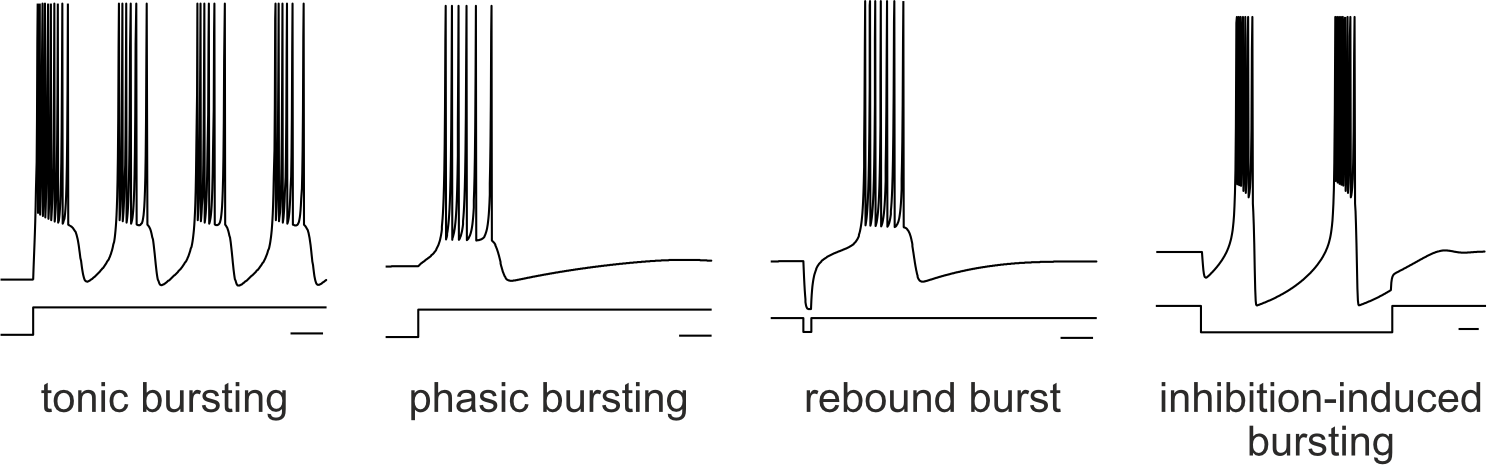
\includegraphics[width=0.85\linewidth]{../img/modelling_r5/examples/classification_of_intrinsic_bursters.png}
    \caption[Classification of intrinsically bursting neurons by neuro-computational features]{
        Classification of intrinsically bursting neurons by neuro-computational features.
        Adapted from \cite{izhikevichDynamicalSystemsNeuroscience2006}, with modifications.
        Electronic version of the figure and reproduction permissions
        are freely available at \url{www.izhikevich.com}.
    }
    \label{fig:classification_intrin_burst}
\end{figure}



\color{red}
Bursting can be classified by:
\begin{itemize}
    \item Modulation of external current
\end{itemize}    

\begin{itemize}
    \item External input
    \begin{itemize}
        \item Tonic bursting
        \item Phasic bursting
        \item Rebound bursting
        \item Inhibition-induced bursting
    \end{itemize}
\end{itemize}


Activation of dSFB Neurons -> increased SWA in R5. dSFB are inhibitory...
\color{black}

Electrophysiological orecordings of R5 neurons in \textit{Drsophila melanogaster}
revealed

\subsection{Phantom Bursting}

The ideas behind previous sections were based on decomposition of the
dynamical system into slow and fast subsystems. However, firstly, existance
of such subsystemts is not a necessary condition to achieve bursting and
not all bursting systems can be decomposed into slow and fast subsystems.

\color{red}

\begin{itemize}
    \item Can be more than one slow variable
    \item More complex dynamics in the phase space
    \item Hedgehog limit cycles (Hedgehog limit cycle attractor)
    \item 
\end{itemize}

\color{black}

%%%%%%%%%%%%%%%%%%%%%%%%%%%%%%%%%%%%%%%%%%%%%%%%%%%%%%%%%%%%%%%%%%%%%%%%%%%%%%%%%
\subsection{Other Types of Bursting}

%%%%%%%%%%%%%%%%%%%%%%%%%%%%%%%%%%%%%%%%%%%%%%%%%%%%%%%%%%%%%%%%%%%%%%%%%%%%%%%%%
\subsection{Summary}


\end{document}